%*****************************************
\chapter{From tissue to single cell transcriptomics, a paradigm shift}\label{ch:singlecell}
%*****************************************
\section{Spatially referenced single cell-like in-situ hybridization data}\label{sec:single_cell_insitu}
  \subsection*{Dividing images into "cells"}
  Because in-situ hybridization keeps the studied tissue spatially untouched, achieving single cell gene expression resolution from one image obtained through fluorescent microscopy is a matter of microscope performance and cell size. For big enough cells, single cell resolution has been documented as far as 1989 \cite{tautz89} with some work specifically directed towards achieving this single cell resolution \cite{poulsen93}.\\
  
  When considering \cite{Tomer10} dataset, with current microscope technology, achieving single cell level resolution in \platy{}'s brain on one particular image is feasible. However, our main limitation is the quantity of data involved, indeed, each brain is separated into 20 slices, for 169 genes. This technical bottleneck can be overcome with an automated way of analysing the fluorescence images. However this is not an easy task, as the computer program required needs to be able to ``see" and divide the global picture into cells. Considering that all cells do not exhibit the same shape and size, constructing this ``cell model" is a very complicated task.\\
  
  Possibilities exit to highlight the limits of the cells and to automatically acquire those boundaries through computer vision. They rely on targeting proteins in the membrane or in the extracellular matrix of the cells with specific fluorescent probes. Once the boundaries are acquired, defining every cell is a matter of finding enclosed spaces. To that end, numerous contour detection algorithms exist \cite{li95,fan01,arbelaez11}.\\
  
  Unfortunately, a dataset with the cells limits highlighted does not yet exist for \platy{}'s brain, making a precise division of the images into cells very difficult. Instead, Tomer used a basic approach to divided the images, the ``cube" model \cite{Tomer10}.


  \subsection*{A simple cell model, the "cube" data}
  
  Every slice of \platy{}'s brain being aligned onto the reference gene scaffold (see section \ref{sec:gene_expression_lab}) for all 169 genes, the ``cube" model simply consists in dividing each image into square approximately the size of an average cell. In our dataset, the size chosen was 3 \microm{2}. Importantly, this is actually smaller than the average cell size in \platy{}'s brain. each slice of the brain being approximately 3 \microm{} thick, the resulting dataset, referenced on a 3-dimensional axis, will contain 3 \microm{3} cubes, each of those attached to the luminescence data for 169 genes.\\
  
  Of course this cell model is far from perfect, it assumes that every cell in the brain are roughly the same size and cubical, which is clearly not the case. Consequently, the ``cube" model will introduce errors in the dataset. The first type of error occurs within areas where the genes under study are highly expressed. In that case, the florescence my contaminate the cubes around that do not necessarily express the same gene see figure \ref{fig:cubeserrors}A. The second type of error is introduced by the choice of 3 \microm{3} cubes. As they are smaller than the average cell, some cubes will fall on areas that may be artificially empty. Indeed, transcription in the cells mainly happens in the nucleus, mRNA then travel in the cytoplasm to be translated but they are not evenly distributed across the cell, in particular for some large cells, parts of the cytoplasm may record no expression in a cell that actually contains a lot of transcripts, see figure \ref{fig:cubeserrors}B.\\
  
  Hence the data will tend to show some discontinuity and inconsistency spatially. With that fact in mind, any method hat we develop using this data, will have to take into account this spatial discontinuity and try as much as possible to smooth over those potential expression gaps.\\
  
    \begin{figure}[bth]
\centerline{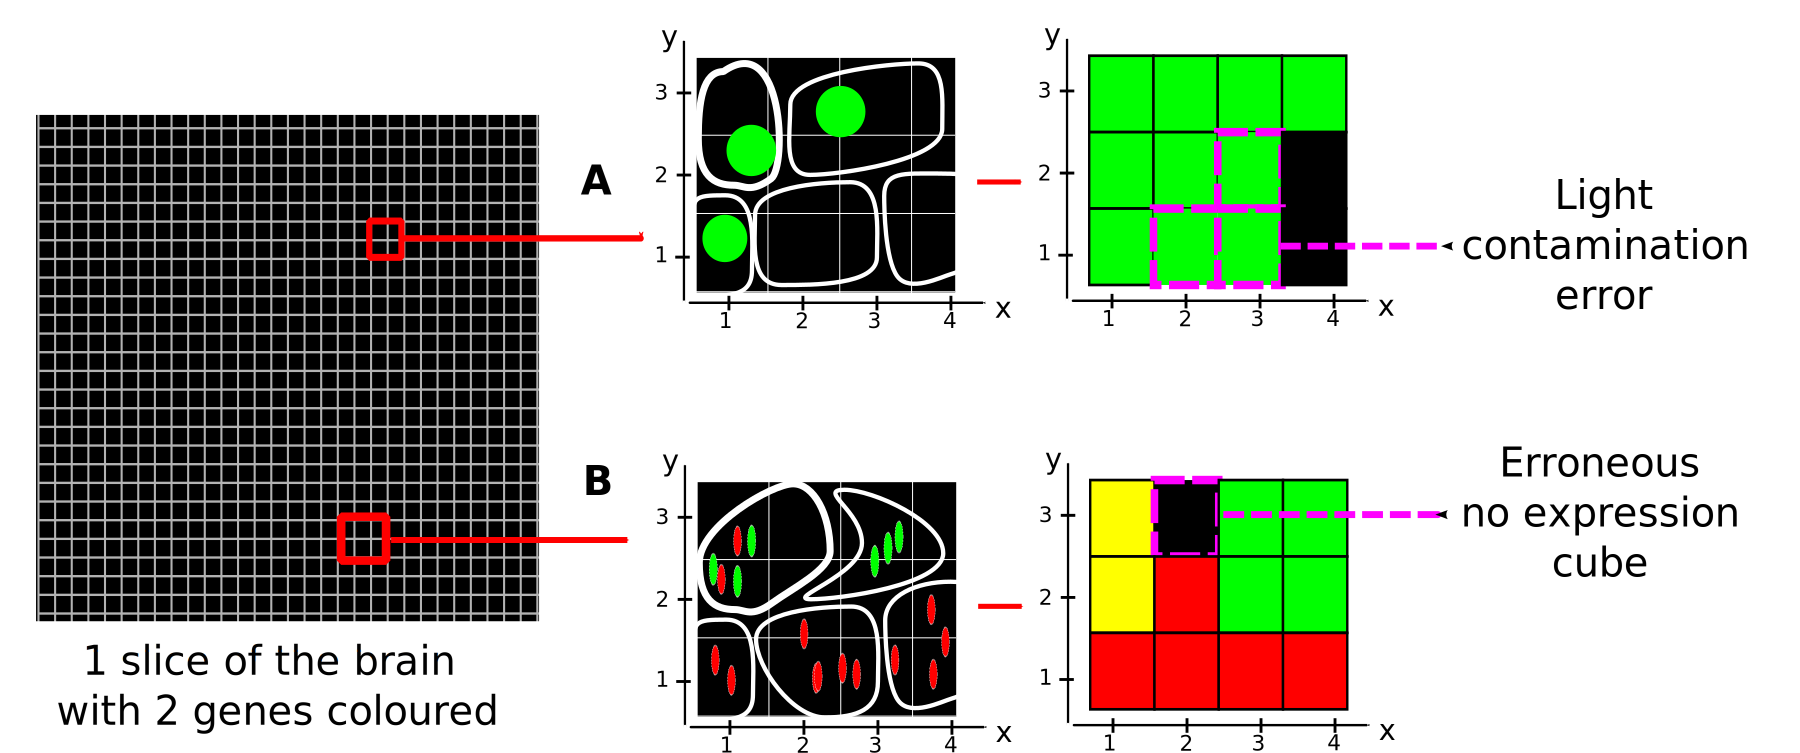
\includegraphics[width=0.9\linewidth]{gfx/chapter2/cubeserrors.png}}
\caption{Errors introduced by the ``cube" cell model. Path A shows how regions with highly expressed genes can introduce errors through light contamination. Path B shows how .}\label{fig:cubeserrors}
	\end{figure}
	
	However, even with this simple cell model the data generated by \cite{Tomer10} is highly valuable. Indeed, not only does this dataset give a snapshot of gene expression for 169 genes in the full brain of \platy{}, it also attaches spatial information to each data point.\\

\section{Singe cell RNA sequencing, building a map of the full transcriptome}\label{sec:single_cell_rnaseq}
  \subsection*{Sequencing single cell RNA contents}
	The scale shift from tissue to single cell is harder to achieve in the case of RNA-seq. As described in the previous section \ref{sec:gene_expression_lab}, an important factor for the success of RNA-seq assays is the starting input quantity of RNA to be sequenced. Taking mammalian cells as a reference, the quantity of RNA depends a lot on the cell type considered and can vary between 10 and 30 pg per cell, only 2\% of which is mRNA \cite{iscove02,islam11}. With such a small input quantity, distinguishing biological variation between different cells from the technical variation linked to cDNA amplification protocols has long been impossible to achieve.\\

	However, with the creation of new protocols \cite{ramskold12,tang09}, and the rise of microfluidics protocol to faciliate the extraction and sequencing of single cells \cite{ozsolak10}, the last couple of years have seen a dramatic increase in the number of single cell RNA-seq based studies \cite{islam13,marinov13,yan13,staahlberg13,deng14}. Challenges remain to be able to analyse further complex tissues from whole transcriptomes obtained from single cell RNA-seq, one of which is the loss of spatial reference induced by the current protocols.

  \subsection*{Mapping back gene expression to a spatial reference}

	Single cell RNA-seq achieves to capture a snapshot of the entire transcriptome of a given cell at a given point in time. However, to analyse cells from a complex tissue, current protocols require that the tissue is reduced to a suspension of single independent cells. This prevents from keeping track of any spatial information about the cells. Hence, when analysing single cell RNA-seq data from a complex tissue, we need to be able to map back every cell to its original location.\\ 
	
	In order to achieve this back-mapping, a reference is needed. This reference should consist in an independent assay where gene expression in the considered tissue is defined for enough genes at a small enough resolution spatially to find for each sequenced cell, if not the exact original location of the cell, at least a spatially restricted region of the brain from which the sequenced cell originated with a high probability.\\
	
	Fortunately, in-situ hybridization assays provide exactly this type of data and we will present in the last section of this chapter \ref{sec:back_mapping_platy} a methodological proof-of-concept of this back-mapping in the brain of \platy{} with 72 sequenced single cells.

\section{About the quantitative trait of single cell expression data}\label{sec:quantitative_single_cell}
  \subsection*{Light contamination in in-situ hybridization data}
  The fluorescence value obtained from in-situ hybridization assays can be considered as quantitative \cite{dorresteijn90}. Indeed, the light intensity emitted by every cell in the considered tissue is correlated with the number of RNA fragments present in the cell as each fragment bound to a probe is an independent sources of emission and the probes are hybridized in the cells in large excess. This means that if the targeted gene is highly expressed in a cell, there will be more sources of emission, thus making the overall light intensity captured on this area higher than on a cell expressing the gene at a low level. \\
  
  As mentioned in a previous section \ref{sec:single_cell_insitu}, in-situ hybridization assays at the single cell level are prone to punctual errors due to the cell model. One of the culprit for those errors, as shown on figure \ref{fig:cubeserrors}B is the phenomenon of light contamination. When a large group of neighbouring cells express the same gene, because of the additivity of light intensity mentioned above, even though the cells express the gene at the same rate, cells surrounded by a lot of other cells expressing the same gene will have an abnormally high light intensity reading due to light contamination from the adjacent areas. As a result, when considering an hypothetical circular portion of tissue where a gene is monotonously expressed, the recorded light intensity will show a gradient with the maximum localized on the circle's centre.\\
  
   \begin{figure}[bth]
\centerline{\includegraphics[width=\linewidth]{gfx/chapter2/whybina.png}}
\caption{{\bf Light contamination on in in-situ hybridization luminescence data seen on the example of gene Ascl.} Panel A shows the raw fluorescent microscopy capture of the gene's expression for one layer in the brain of \platy{}. Panel B shows the light intensity measured along the red line in panel A. Because of the small scale of study, cells surrounded by other cells expressing the same gene will have a higher intensity values because of nearby light contamination. Even though there might be an actual gradient in the expression level bewteen the cell in the middle and the others there is no option to separate it from the light contamination component.}\label{fig:why_binarize}
	\end{figure}
  
  As shown on figure \ref{fig:why_binarize}, we can confirm that light contamination issue on the in-situ hybridization data in \platy{}'s brain. In that context, and because of the single cell scale of our study, considering the in-situ hybridization data as quantitative may have introduced significant errors. In order to avoid this light contamination bias we decided to transform the quantitative data set into a binary data set where for a given ``cube", genes are simply expressed or not. The binarization method is described in the following section \ref{sec:binarizing}.
  


  \subsection*{Technical noise in single cell RNA-seq data}
    - FIG 6 : show "typical" correlation plot from single cell RNA-seq with the noise increasing when reducing starting material
    - Both methods are currently unreliable quantitatively => need to binarize

\section{Binarizing gene expression datasets}\label{sec:binarizing}
  \subsection*{Binarizing in-situ hybrdization datasets}
	As shown in Figure \ref{fig:why_binarize} and discussed in the previous section \ref{sec:quantitative_single_cell}, we decided to avoid the various problems linked to light contamination by transforming the ``quantitative" fluorescence information into binary data. In other words, if $S$ is the set of all ``cubes" in the brain, $M$ the set of all the considered genes and $y_{i,m}$ the value retrieved from the in-situ hybridization data for ``cube" $i \in S$ and gene $m \in M$, then  $y_{i,m} = 1$ if gene $m$ is expressed at site $i$, $y_{i,m} = 0$ otherwise. The binarization process itself is not trivial. Indeed, defining the light intensity threshold above which a gene is considered expressed is a complicated problem, especially for noisy data.\\

	Looking at the density of intensities across cubes for each gene, we found two very different scenarios: some densities were separated into two clear peaks, making the threshold easy to find while others exhibited a single peak making it hard to find a clear cut value as shown in figure \ref{fig:densities_bina}. After trying different thresholding methods based on those densities, we found that the resulting binary expression was not satisfying for a large number of genes. Considering that this binarized dataset will be the cornerstone of the work presented in this thesis, it was very important to achieve a high confidence thresholding. Given the small number of genes studied (169), and the collaboration with a team of biologist working specifically on \platyfull{}'s brain, we decided to opt for a manual approach to thresholding. Indeed, by going through the 169 genes one by one, and adjusting the threshold manually until the resulting binarized expression patter corresponded perfectly to 1) the fluorescent stack images from in-situ hybridization data; 2) the biologically known expression patterns in the brain of \platy{} validated by the biologists.\\
	
	\begin{figure}[bth]
\centerline{\includegraphics[width=\linewidth]{gfx/chapter2/densities_bina.png}}
\caption{Light intensity densities found for genes rOpsin and PRDM8.H92 accross \platy{}'s whole brain on a logaritmic scale. $N$ for each graph is the number of ``cubes" in the dataset where the fluorescence value is higher than $0$. On the one hand, the log density shows two clear peaks for rOpsin, making the choice of a expression threshold easy. PRDM8.H92 on the other hand does not display such a clear cut threshold.}\label{fig:densities_bina}
	\end{figure}
	
	This method resulted in a high confidence binarized dataset for $86$ genes. Several reasons explain why $83$ genes out of the starting $169$ were removed from the dataset. For some of the genes no good threshold could be found, this was due to high noise level in the in-situ hybridization images. Other images suffered from experimental errors resulting in blurred and unexploitable expression patterns. Finally some images where polluted by a well known experimental artefact linked to fluorescent microscopy imaging.\\
	
	Although the aforementioned method resulted in a high quality binary dataset, it has been possible only because the number of genes considered was small. This will not be the case when dealing with RNA-seq data.
	


  \subsection*{Binarizing whole transcriptomes}
    - Manual curation no longer possible
    - Thresholding ideally with density peaks
    - Problems that may occur and possible solutions (figure?)

\section{Preliminary results on mapping single cell RNA-seq data in from Platynereis' brain}\label{sec:back_mapping_platy}
  \subsection*{Single cell RNA-seq in Platynereis' brain}
  
    	Collaborations with the Kaia Achim in the Detlev lab in EMBL as well as Luis R. Saraiva in the Marioni lab have allowed us to get 72 single cells from \platy{}'s 48hpf developing brain sequenced. The method used was the Tang protocol \cite{tang09} within a microfluidics pipeline \todo{get info on sequencing}.\\
  	
	Of course those results do not include the spatial localization of the cells. As a crucial point in any dowstream analysis, we need to be able to map back the single cells to their original location in the brain. To that end, we took advantage of the spatially localized in-situ hybridization described in the previous section.\\
	
    - Present the data (number of cell)
    - Present the method used (to dissolve the brain, to capture the cells, to sequence the cells
  \subsection*{Mapping back RNA-seq data back to PrimR in-situ hybridization assays}
  	We started by mapping the RNA-seq reads to the 169 reference genes composing the in-situ hybridization data using Bowtie.\todo{cite nuno pipline}. The resulting dataset is a the count number for each of the 169 genes in the 71 cells sequenced. In order to map back to the in-situ hybridization data, our approach consisted in extracting the genes that were the most specifically expressed for each sequenced cell, then compare this specific fingerprint to the in-situ 3D data to isolate the regions of the brain where those specific genes are co-expressed.\\
	
	The goals of this study were to validate the protocol used in order to obtain single cell RNA-seq results in \platy{}'s brain and to establish a methodological proof-of-concept on spatially mapping RNA-seq results onto in-situ hybridization data. We will present here a few examples of sequenced cells, their most specifically expressed genes, their resulting potential original location in the brain and the probable cell type they belong to.\\
    - Select the overlapping genes
    - Present mapping method (Nuno's pipeline)
    - Present simple mapping technique and why it is not satisfactory
    - Present John's method  
    - FIG 6: find a nice way to show a few good examples of mapping

%*****************************************
%*****************************************
%*****************************************
%*****************************************
%*****************************************
